\documentclass[11pt]{article}
\usepackage[margin=1in]{geometry}
\usepackage{graphicx}
\usepackage{booktabs}
\usepackage{longtable}
\usepackage{array}
\usepackage{hyperref}
\usepackage{pdflscape}
\usepackage{enumitem}
\usepackage{caption}
\graphicspath{{figures/}}
\hypersetup{colorlinks=true,linkcolor=blue,urlcolor=blue}
\setlength{\LTpre}{0.35em}
\setlength{\LTpost}{0.5em}
\title{SLR 1: Questions 1--3}
\author{}
\date{}

\begin{document}
\maketitle

\section{Protocol basis and scope of this report}
The protocol research questions are:
\begin{enumerate}[leftmargin=*]
\item RQ1. How can nanosatellite missions and EPS be modeled in a general manner with minimal knowledge about their behavior?
\item RQ2. What are the claimed outcomes related to reliability, reproducibility, and integrability derived from EPS modeling in nanosatellite missions?
\item RQ3. How have verification procedures been integrated into EPS models prior to physical development?
\end{enumerate}

The protocol extraction fields used as the organizing frame are: Bibliographic metadata, Modeling scope (system-level, EPS-level, requirements, architecture, budget, verification, etc.), MBSE language / method / tool, Research question(s) addressed, Claimed outcomes, Verification / validation linkage, Key findings, Limitations / gaps.  The corpus summarized here contains 40 accessible extracted studies (21 core and 19 supporting), from 2013--2025.  The four inaccessible kept corpus records listed in \texttt{pdf-status.md} are not included in the extraction synthesis.

\section{Search, screening, retrieval, and extraction flow}
Figure~\ref{fig:prisma} gives the PRISMA-style flow reconstructed from the maintained search, screening, retrieval, and extraction artifacts.

\begin{figure}[htbp]
\centering
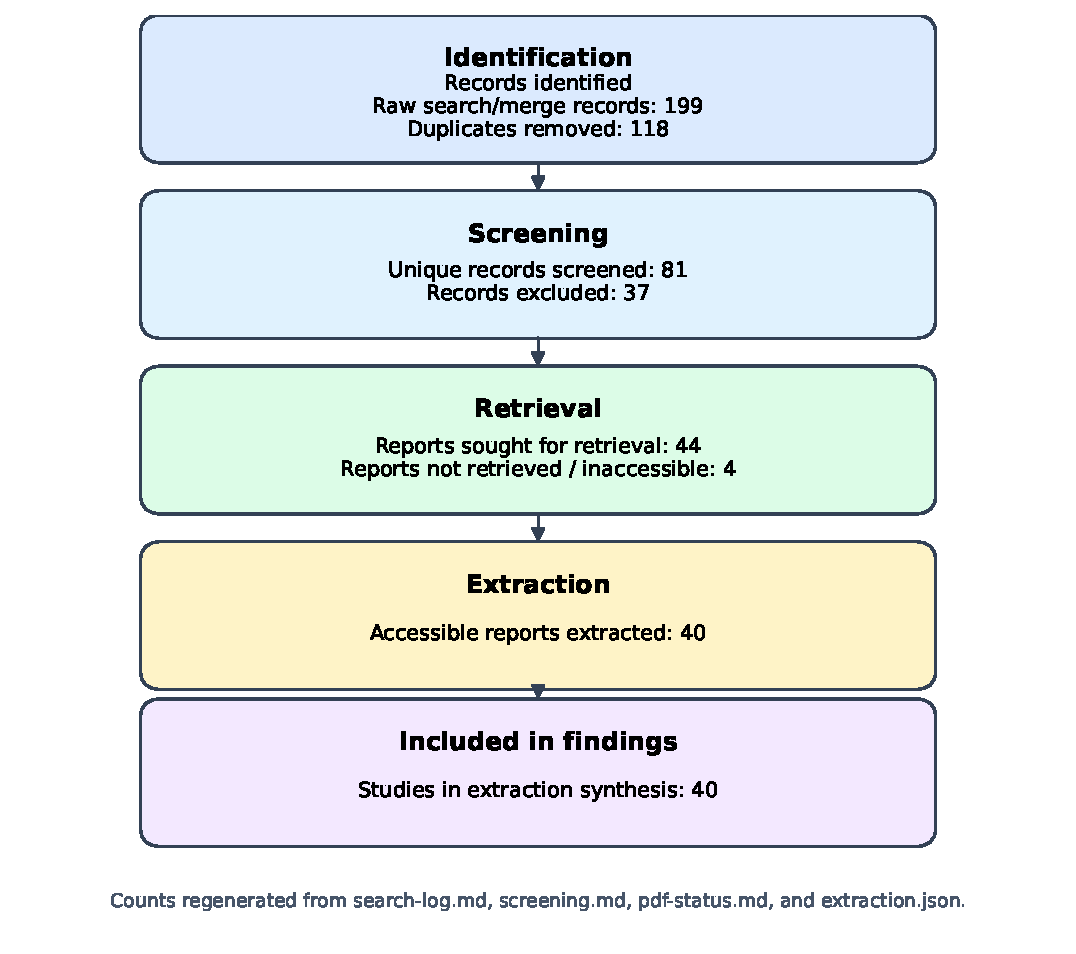
\includegraphics[width=0.88\linewidth]{prisma_flow.pdf}
\caption{PRISMA-style flow for SLR1 extraction synthesis.}
\label{fig:prisma}
\end{figure}

The regenerated flow is: 199 raw merged search records, 118 duplicates removed, 81 unique records screened, 37 excluded during screening, 44 reports sought for retrieval, 4 not retrieved/inaccessible, and 40 extracted.

\begin{figure}[htbp]
\centering
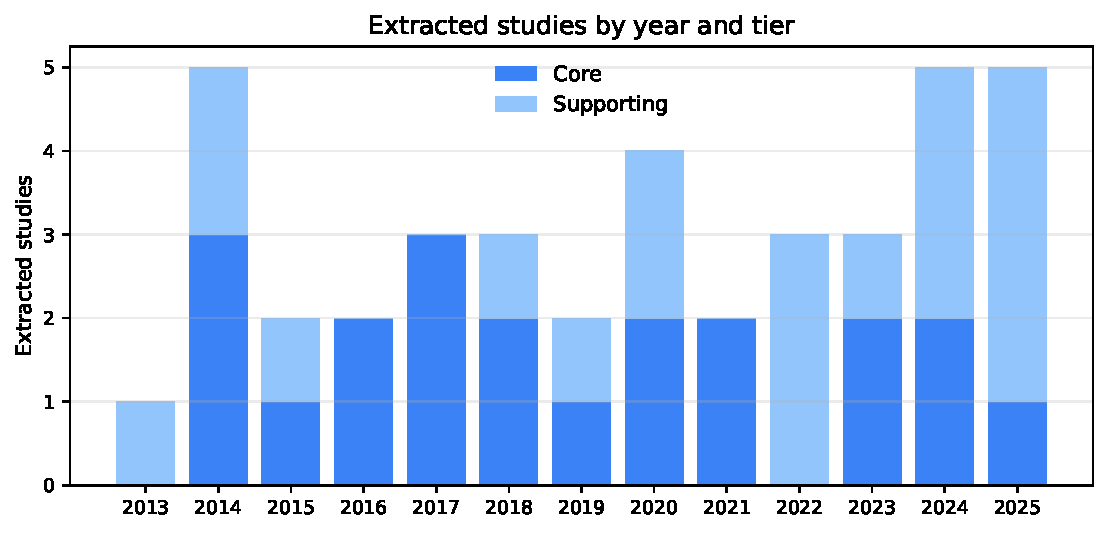
\includegraphics[width=0.95\linewidth]{year_tier_counts.pdf}
\caption{Extracted studies by publication year and screening tier.}
\end{figure}

\begin{figure}[htbp]
\centering
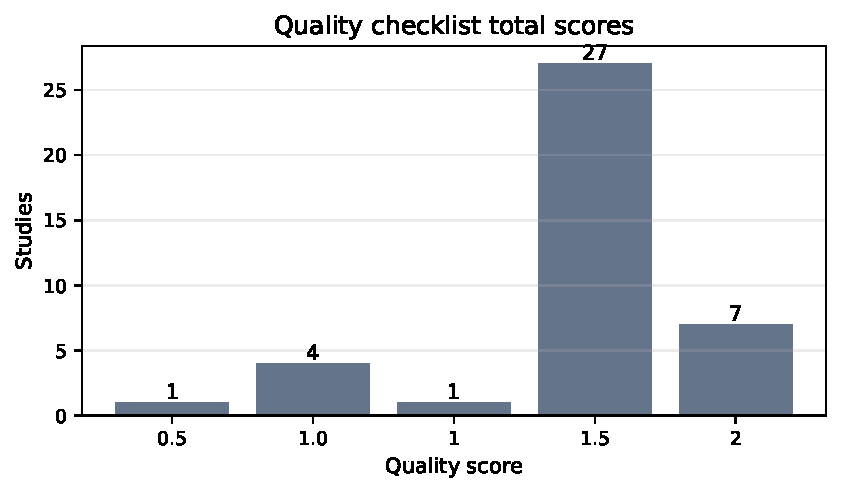
\includegraphics[width=0.72\linewidth]{quality_score_counts.pdf}
\caption{Quality checklist total scores recorded during extraction.}
\end{figure}

\section{RQ relevance and modeling focus}
Figure~\ref{fig:rq-counts} summarizes the extraction-coded relevance to each protocol RQ.  The key pattern is that RQ2 is coded as partial for all extracted studies, reflecting that claimed outcomes are usually MBSE/process claims rather than direct measured EPS reliability, reproducibility, or integrability outcomes.  RQ3 has the smallest ``yes'' subset.

\begin{figure}[htbp]
\centering
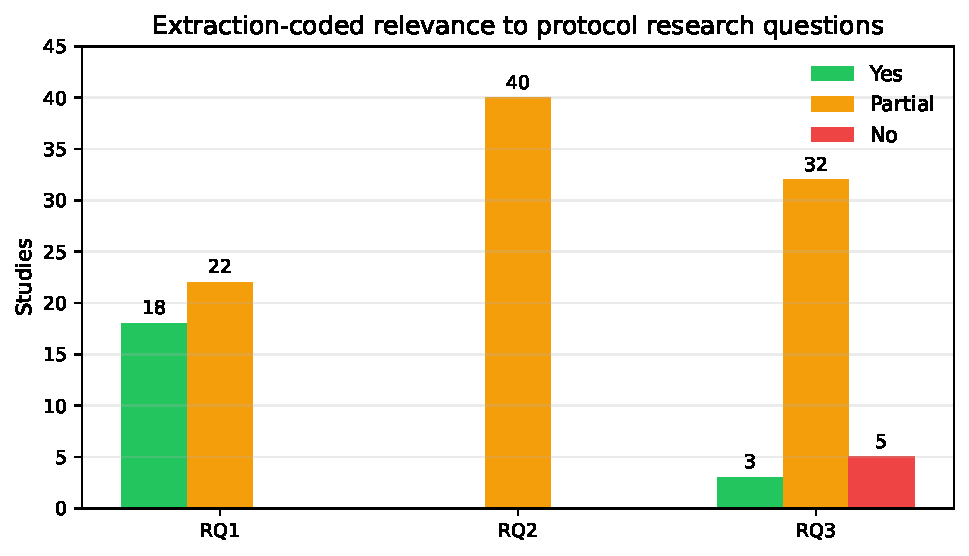
\includegraphics[width=0.78\linewidth]{rq_relevance_counts.pdf}
\caption{Extraction-coded relevance to each protocol research question.}
\label{fig:rq-counts}
\end{figure}

\begin{figure}[htbp]
\centering
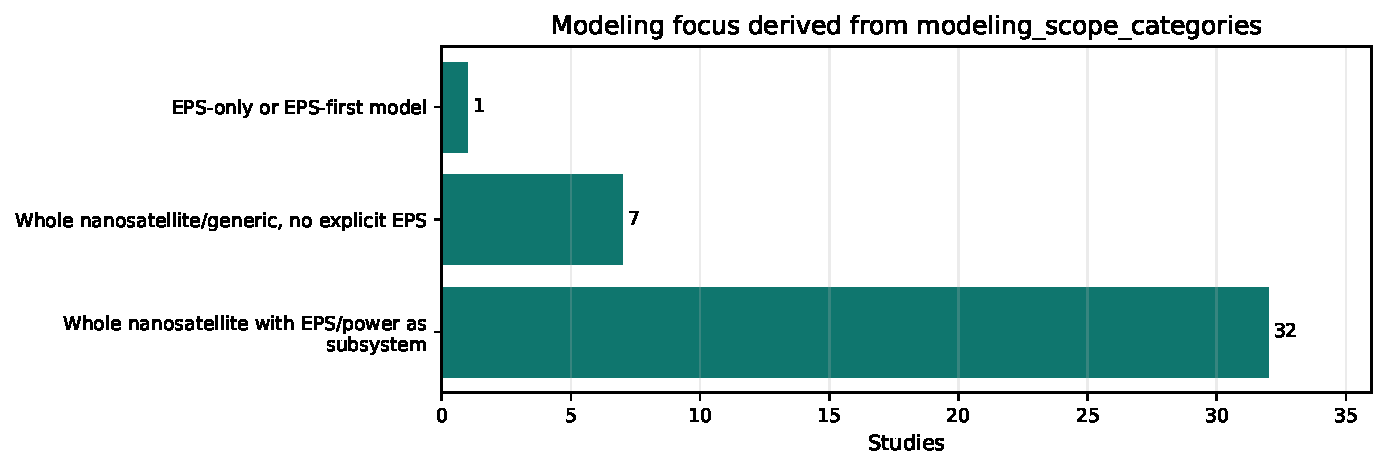
\includegraphics[width=0.82\linewidth]{model_focus_counts.pdf}
\caption{Modeling focus derived deterministically from \texttt{modeling\_scope\_categories}.}
\label{fig:focus-counts}
\end{figure}

The focus categories answer the user's requested distinctions directly from extraction categories:
\begin{itemize}[leftmargin=*]
\item Whole nanosatellite with EPS/power as a subsystem: 32 studies.
\item Whole nanosatellite/generic with no explicit EPS: 7 studies (paper-0010, paper-0002, paper-0034, paper-0024, paper-0068, paper-0071, paper-0063).
\item EPS-only or EPS-first model: 1 study (paper-0026).
\end{itemize}

\begin{figure}[p]
\centering
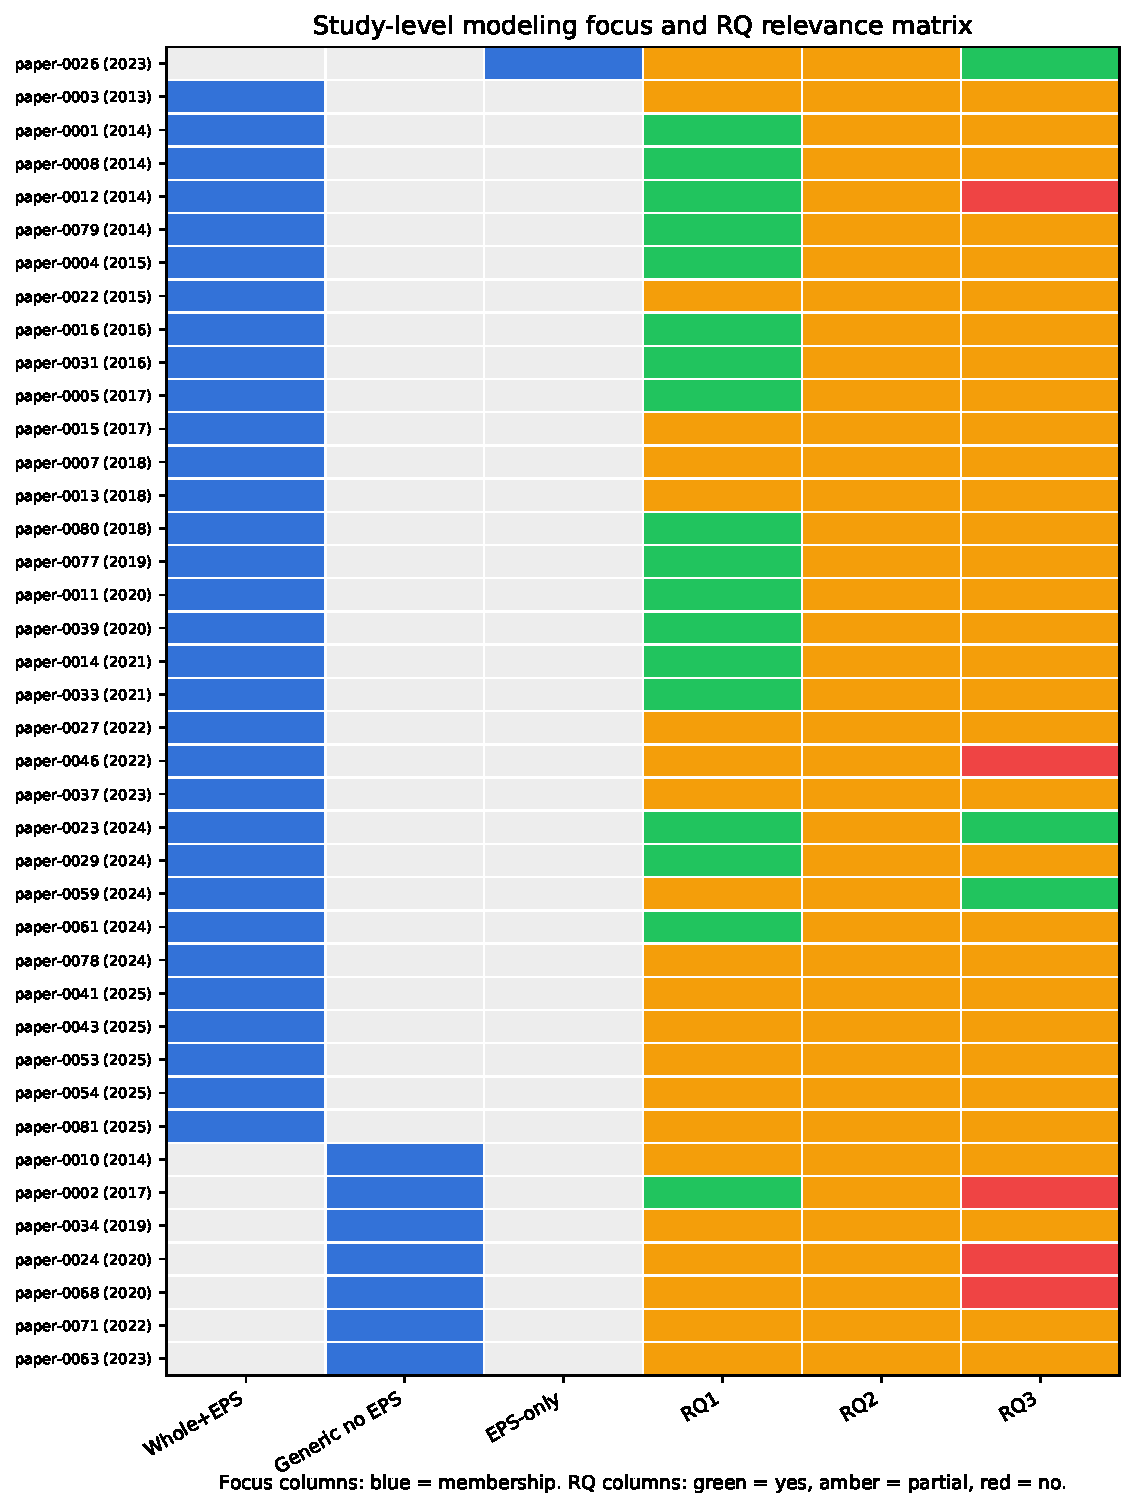
\includegraphics[width=0.82\linewidth]{study_focus_rq_matrix.pdf}
\caption{Study-level matrix showing modeling focus membership and RQ relevance.}
\label{fig:study-matrix}
\end{figure}

\subsection{Which studies fall in each modeling-focus group}
\begin{longtable}{p{0.27\linewidth}p{0.10\linewidth}p{0.55\linewidth}}
\toprule Focus & Count & Studies \\
\midrule\endfirsthead
\toprule Focus & Count & Studies \\ \midrule\endhead
Whole nanosatellite with EPS/power as subsystem & 32 & paper-0003 (2013); paper-0001 (2014); paper-0008 (2014); paper-0012 (2014); paper-0079 (2014); paper-0004 (2015); paper-0022 (2015); paper-0016 (2016); paper-0031 (2016); paper-0005 (2017); paper-0015 (2017); paper-0007 (2018); paper-0013 (2018); paper-0080 (2018); paper-0077 (2019); paper-0011 (2020); paper-0039 (2020); paper-0014 (2021); paper-0033 (2021); paper-0027 (2022); paper-0046 (2022); paper-0037 (2023); paper-0023 (2024); paper-0029 (2024); paper-0059 (2024); paper-0061 (2024); paper-0078 (2024); paper-0041 (2025); paper-0043 (2025); paper-0053 (2025); paper-0054 (2025); paper-0081 (2025) \\
Whole nanosatellite/generic, no explicit EPS & 7 & paper-0010 (2014); paper-0002 (2017); paper-0034 (2019); paper-0024 (2020); paper-0068 (2020); paper-0071 (2022); paper-0063 (2023) \\
EPS-only or EPS-first model & 1 & paper-0026 (2023) \\
\bottomrule\end{longtable}

\subsection{Generic whole-nanosatellite studies that do not model EPS explicitly}
Table~\ref{tab:generic-no-eps} lists the generic/no-EPS studies and the extraction-based reason each is not counted as EPS modeling.
\begin{longtable}{p{0.14\linewidth}p{0.30\linewidth}p{0.46\linewidth}}
\caption{Why generic system-level studies were not counted as explicit EPS modeling.}\label{tab:generic-no-eps}\\
\toprule Study & Short title & Why it is generic/no-EPS \\
\midrule\endfirsthead
\toprule Study & Short title & Why it is generic/no-EPS \\ \midrule\endhead
paper-0010 & Small Satellite Systems Design Methodology: A Formal and Agile... & formal/agile small-satellite design process and formal-methods V\&V, not a subsystem model \\
paper-0002 & A Model-Based Systems Engineering (MBSE) Approach for Defining... & behavior/use-case and functional decomposition of a generic CubeSat mission, not subsystem power design \\
paper-0034 & Requirements Modeling Language and Automated Testing for CubeSats & requirements modeling language and automated-testing/traceability method, not a power subsystem model \\
paper-0024 & Analysis of MBSE/PLM Integration: From Conceptual Design to... & MBSE--PLM information-flow analysis from conceptual to detailed design, not EPS architecture \\
paper-0068 & Digital Engineering Information Exchange Model for Space... & digital-engineering information-exchange/DSM--DMM mapping for mission architecture, not EPS \\
paper-0071 & A Model-Based Approach to Risk Management for RVSAT-1: a... & SysML risk-management model for a student nanosatellite, not EPS design or verification \\
paper-0063 & Development of a Nanosatellite System Modeling Architecture... & nanosatellite system-modeling architecture with a communications-subsystem V\&V demonstrator, not EPS \\
\bottomrule\end{longtable}

\section{Categories arising in extraction fields}
\subsection{Modeling-scope categories}
\begin{figure}[htbp]
\centering
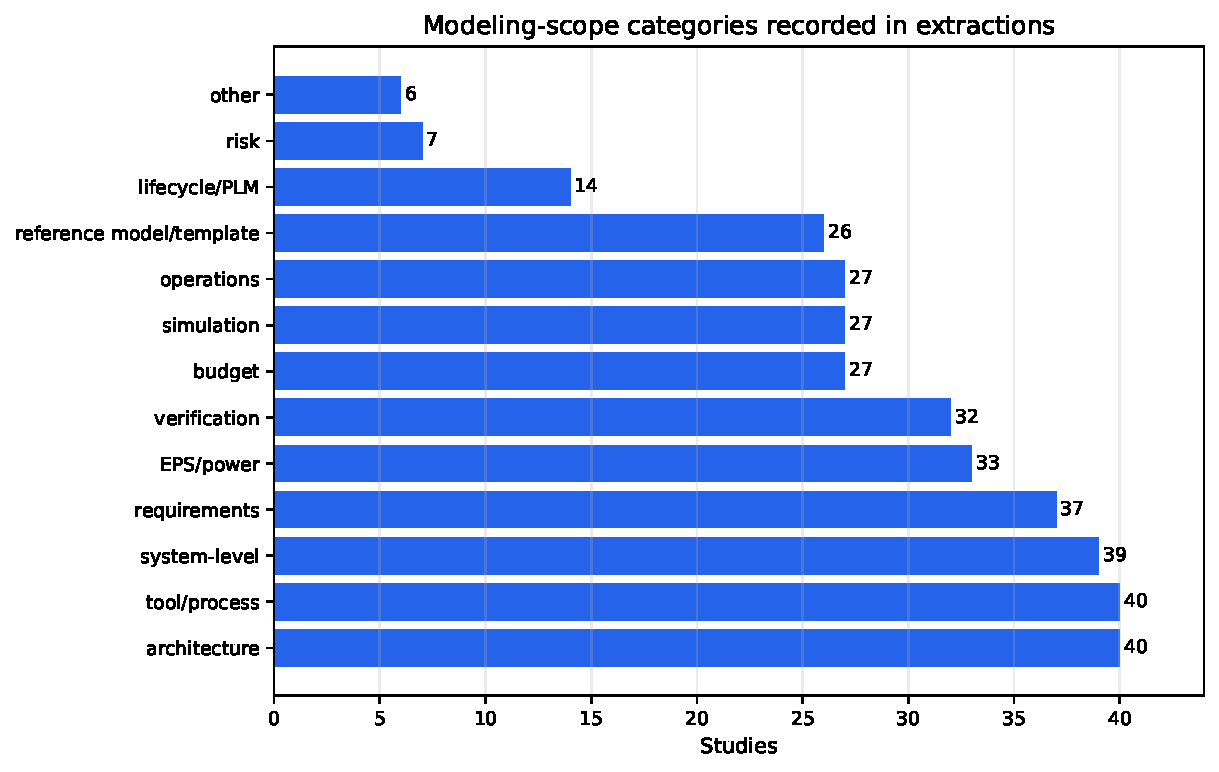
\includegraphics[width=0.90\linewidth]{modeling_scope_categories.pdf}
\caption{Multi-label modeling-scope categories recorded in the standardized extractions.}
\end{figure}

\begin{longtable}{p{0.48\linewidth}r p{0.34\linewidth}}
\toprule
Category & n & Study IDs \\
\midrule
\endfirsthead
\toprule Category & n & Study IDs \\ \midrule \endhead
architecture & 40 & paper-0001, paper-0002, paper-0003, paper-0004, paper-0005, paper-0007, paper-0008, paper-0010, paper-0011, paper-0012, paper-0013, paper-0014, paper-0015, paper-0016, paper-0022, paper-0023, paper-0024, paper-0026, paper-0027, paper-0029, paper-0031, paper-0033, paper-0034, paper-0037, paper-0039, paper-0041, paper-0043, paper-0046, paper-0053, paper-0054, paper-0059, paper-0061, paper-0063, paper-0068, paper-0071, paper-0077, paper-0078, paper-0079, paper-0080, paper-0081 \\
tool/process & 40 & paper-0001, paper-0002, paper-0003, paper-0004, paper-0005, paper-0007, paper-0008, paper-0010, paper-0011, paper-0012, paper-0013, paper-0014, paper-0015, paper-0016, paper-0022, paper-0023, paper-0024, paper-0026, paper-0027, paper-0029, paper-0031, paper-0033, paper-0034, paper-0037, paper-0039, paper-0041, paper-0043, paper-0046, paper-0053, paper-0054, paper-0059, paper-0061, paper-0063, paper-0068, paper-0071, paper-0077, paper-0078, paper-0079, paper-0080, paper-0081 \\
system-level & 39 & paper-0001, paper-0002, paper-0003, paper-0004, paper-0005, paper-0007, paper-0008, paper-0010, paper-0011, paper-0012, paper-0013, paper-0014, paper-0015, paper-0016, paper-0022, paper-0023, paper-0024, paper-0027, paper-0029, paper-0031, paper-0033, paper-0034, paper-0037, paper-0039, paper-0041, paper-0043, paper-0046, paper-0053, paper-0054, paper-0059, paper-0061, paper-0063, paper-0068, paper-0071, paper-0077, paper-0078, paper-0079, paper-0080, paper-0081 \\
requirements & 37 & paper-0001, paper-0002, paper-0003, paper-0004, paper-0005, paper-0007, paper-0008, paper-0010, paper-0011, paper-0012, paper-0013, paper-0014, paper-0015, paper-0016, paper-0022, paper-0023, paper-0026, paper-0027, paper-0029, paper-0031, paper-0033, paper-0034, paper-0037, paper-0039, paper-0041, paper-0043, paper-0046, paper-0053, paper-0054, paper-0059, paper-0061, paper-0063, paper-0077, paper-0078, paper-0079, paper-0080, paper-0081 \\
EPS/power & 33 & paper-0001, paper-0003, paper-0004, paper-0005, paper-0007, paper-0008, paper-0011, paper-0012, paper-0013, paper-0014, paper-0015, paper-0016, paper-0022, paper-0023, paper-0026, paper-0027, paper-0029, paper-0031, paper-0033, paper-0037, paper-0039, paper-0041, paper-0043, paper-0046, paper-0053, paper-0054, paper-0059, paper-0061, paper-0077, paper-0078, paper-0079, paper-0080, paper-0081 \\
verification & 32 & paper-0001, paper-0003, paper-0004, paper-0005, paper-0007, paper-0008, paper-0010, paper-0011, paper-0013, paper-0014, paper-0015, paper-0016, paper-0022, paper-0023, paper-0026, paper-0027, paper-0031, paper-0033, paper-0034, paper-0037, paper-0043, paper-0053, paper-0054, paper-0059, paper-0061, paper-0063, paper-0071, paper-0077, paper-0078, paper-0079, paper-0080, paper-0081 \\
budget & 27 & paper-0001, paper-0003, paper-0004, paper-0007, paper-0008, paper-0011, paper-0012, paper-0016, paper-0022, paper-0023, paper-0026, paper-0027, paper-0029, paper-0033, paper-0039, paper-0041, paper-0043, paper-0046, paper-0053, paper-0054, paper-0061, paper-0071, paper-0077, paper-0078, paper-0079, paper-0080, paper-0081 \\
simulation & 27 & paper-0001, paper-0003, paper-0004, paper-0005, paper-0008, paper-0010, paper-0011, paper-0012, paper-0015, paper-0016, paper-0022, paper-0023, paper-0027, paper-0029, paper-0031, paper-0033, paper-0041, paper-0043, paper-0046, paper-0053, paper-0054, paper-0059, paper-0061, paper-0063, paper-0078, paper-0079, paper-0080 \\
operations & 27 & paper-0001, paper-0002, paper-0003, paper-0004, paper-0005, paper-0008, paper-0011, paper-0012, paper-0014, paper-0015, paper-0016, paper-0022, paper-0023, paper-0026, paper-0031, paper-0033, paper-0037, paper-0043, paper-0053, paper-0054, paper-0059, paper-0061, paper-0063, paper-0077, paper-0078, paper-0080, paper-0081 \\
reference model/template & 26 & paper-0001, paper-0002, paper-0003, paper-0004, paper-0005, paper-0007, paper-0008, paper-0011, paper-0013, paper-0014, paper-0015, paper-0016, paper-0022, paper-0023, paper-0026, paper-0029, paper-0031, paper-0033, paper-0037, paper-0039, paper-0054, paper-0061, paper-0077, paper-0079, paper-0080, paper-0081 \\
lifecycle/PLM & 14 & paper-0003, paper-0004, paper-0008, paper-0016, paper-0022, paper-0023, paper-0024, paper-0029, paper-0031, paper-0043, paper-0046, paper-0054, paper-0059, paper-0068 \\
risk & 7 & paper-0007, paper-0008, paper-0010, paper-0054, paper-0061, paper-0071, paper-0078 \\
other & 6 & paper-0014, paper-0024, paper-0037, paper-0039, paper-0068, paper-0071 \\
\bottomrule
\end{longtable}

\subsection{MBSE languages, methods, and tools}
The high-level extraction categories show SysML dominance but also a long tail of methods and toolchains.  ``Other'' is present in all extraction files and is omitted from the main high-level tool figure; it remains in \texttt{data/category\_counts.csv}.

\begin{figure}[htbp]
\centering
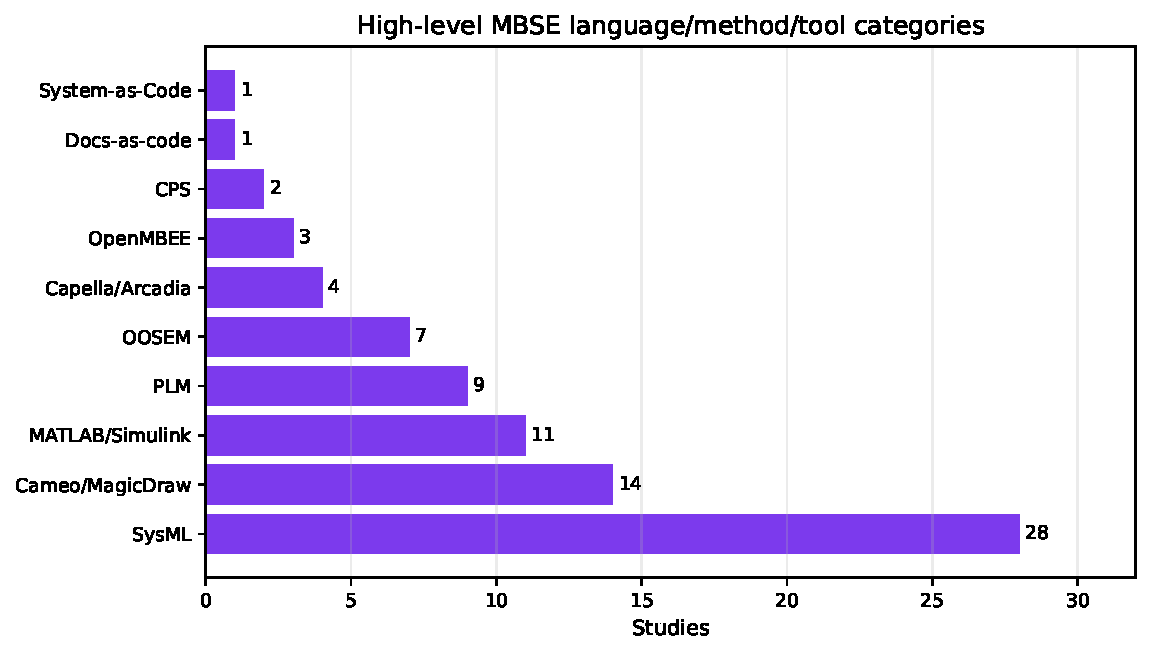
\includegraphics[width=0.78\linewidth]{tool_category_counts.pdf}
\caption{High-level MBSE language/method/tool categories, excluding the uninformative ``Other'' category.}
\end{figure}

\begin{figure}[htbp]
\centering
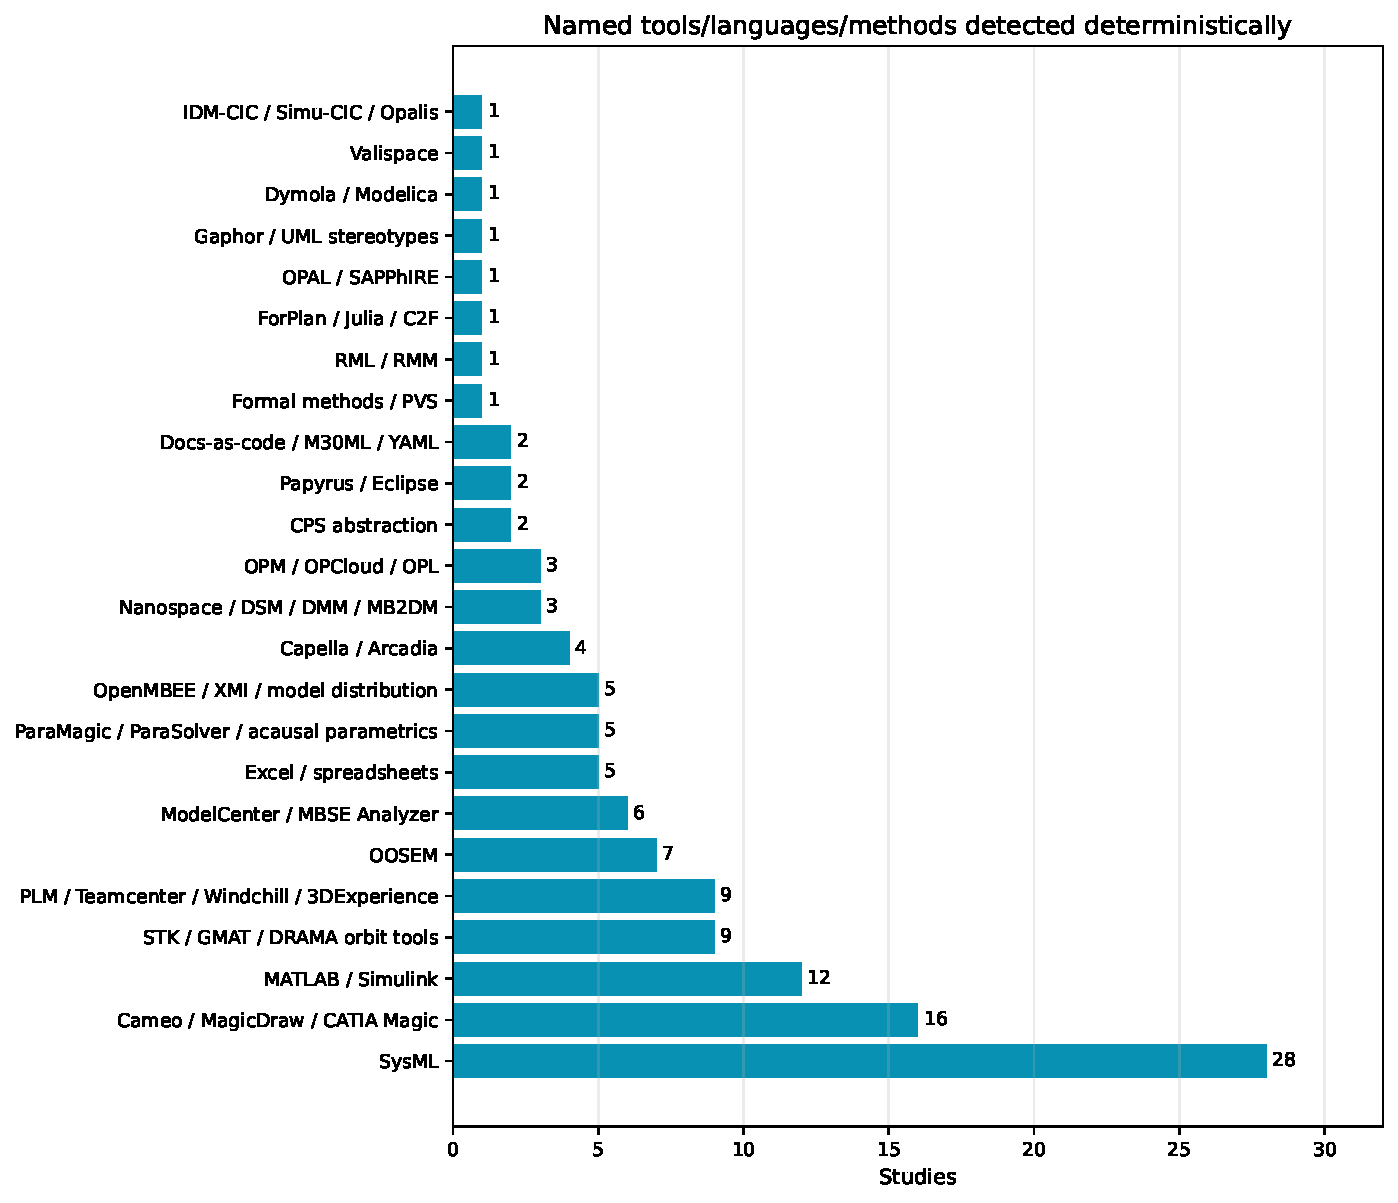
\includegraphics[width=0.92\linewidth]{exact_tool_counts.pdf}
\caption{Named tools/languages/methods detected from \texttt{mbse\_language\_method\_tool} using deterministic keyword rules.}
\end{figure}

\begin{longtable}{p{0.48\linewidth}r p{0.34\linewidth}}
\toprule
Category & n & Study IDs \\
\midrule
\endfirsthead
\toprule Category & n & Study IDs \\ \midrule \endhead
SysML & 28 & paper-0001, paper-0002, paper-0003, paper-0004, paper-0005, paper-0007, paper-0008, paper-0010, paper-0011, paper-0013, paper-0014, paper-0015, paper-0016, paper-0022, paper-0023, paper-0026, paper-0027, paper-0029, paper-0031, paper-0033, paper-0039, paper-0059, paper-0063, paper-0071, paper-0077, paper-0078, paper-0079, paper-0080 \\
Cameo / MagicDraw / CATIA Magic & 16 & paper-0001, paper-0002, paper-0003, paper-0004, paper-0005, paper-0008, paper-0011, paper-0012, paper-0013, paper-0016, paper-0022, paper-0023, paper-0031, paper-0039, paper-0063, paper-0080 \\
MATLAB / Simulink & 12 & paper-0001, paper-0003, paper-0004, paper-0008, paper-0011, paper-0012, paper-0013, paper-0023, paper-0063, paper-0078, paper-0079, paper-0080 \\
STK / GMAT / DRAMA orbit tools & 9 & paper-0001, paper-0003, paper-0004, paper-0008, paper-0011, paper-0013, paper-0054, paper-0061, paper-0078 \\
PLM / Teamcenter / Windchill / 3DExperience & 9 & paper-0004, paper-0008, paper-0016, paper-0022, paper-0024, paper-0031, paper-0046, paper-0059, paper-0068 \\
OOSEM & 7 & paper-0004, paper-0015, paper-0016, paper-0022, paper-0031, paper-0063, paper-0080 \\
ModelCenter / MBSE Analyzer & 6 & paper-0001, paper-0003, paper-0004, paper-0008, paper-0011, paper-0013 \\
Excel / spreadsheets & 5 & paper-0003, paper-0061, paper-0063, paper-0080, paper-0081 \\
ParaMagic / ParaSolver / acausal parametrics & 5 & paper-0003, paper-0004, paper-0008, paper-0079, paper-0080 \\
OpenMBEE / XMI / model distribution & 5 & paper-0013, paper-0016, paper-0022, paper-0031, paper-0077 \\
Capella / Arcadia & 4 & paper-0033, paper-0043, paper-0078, paper-0081 \\
Nanospace / DSM / DMM / MB2DM & 3 & paper-0024, paper-0027, paper-0068 \\
OPM / OPCloud / OPL & 3 & paper-0024, paper-0041, paper-0068 \\
CPS abstraction & 2 & paper-0010, paper-0033 \\
Papyrus / Eclipse & 2 & paper-0026, paper-0071 \\
Docs-as-code / M30ML / YAML & 2 & paper-0037, paper-0081 \\
Formal methods / PVS & 1 & paper-0010 \\
RML / RMM & 1 & paper-0034 \\
ForPlan / Julia / C2F & 1 & paper-0033 \\
OPAL / SAPPhIRE & 1 & paper-0046 \\
Gaphor / UML stereotypes & 1 & paper-0029 \\
Dymola / Modelica & 1 & paper-0059 \\
Valispace & 1 & paper-0061 \\
IDM-CIC / Simu-CIC / Opalis & 1 & paper-0053 \\
System-as-Code / Python / JSON & 1 & paper-0081 \\
\bottomrule
\end{longtable}

\subsection{Claimed outcomes}
Outcome categories are extracted from the \texttt{claimed\_outcomes} lists using deterministic keyword rules and with negated/absence statements separated.  The most frequent positive outcome categories are: Efficiency, automation, or reduced time/cost/effort (32), Integration, interoperability, or data exchange (32), Communication, collaboration, or stakeholder alignment (30), Reuse, templates, standardization, or replicability (27), Traceability, consistency, or single source of truth (27).

\begin{figure}[htbp]
\centering
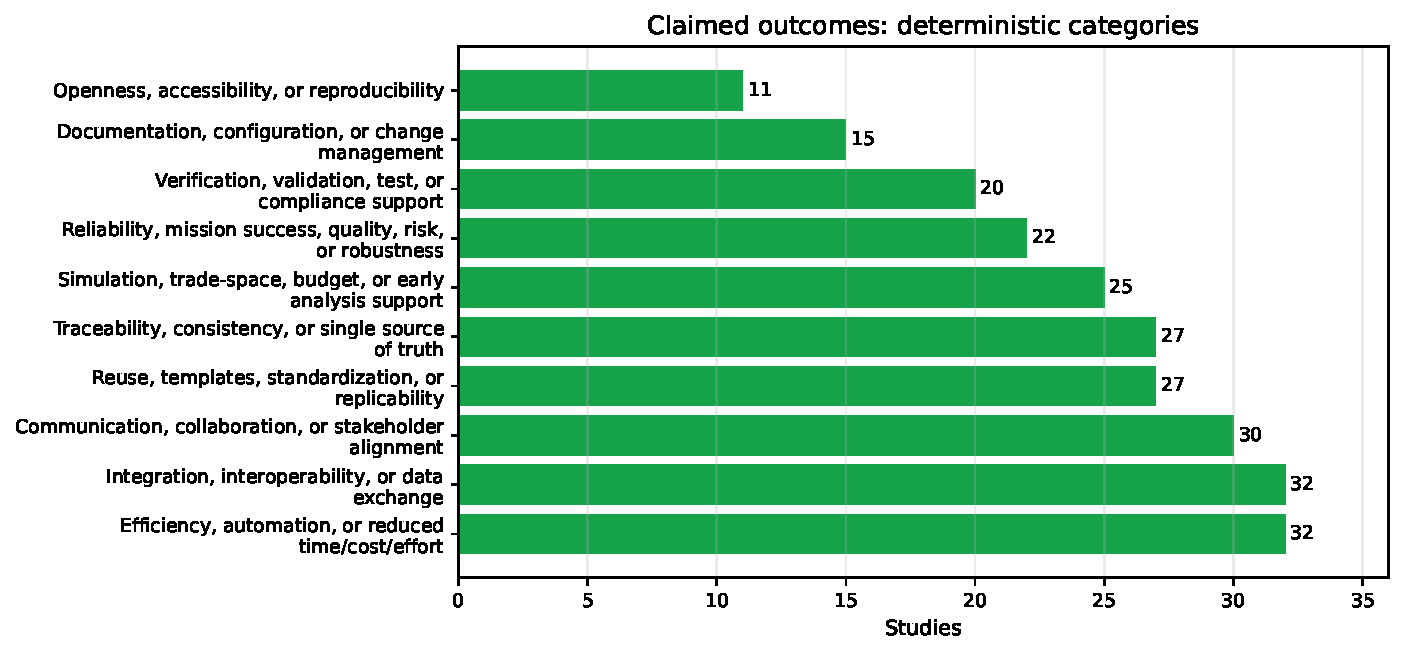
\includegraphics[width=0.92\linewidth]{outcome_categories.pdf}
\caption{Positive claimed-outcome categories detected in the extraction field.}
\end{figure}

\begin{figure}[htbp]
\centering
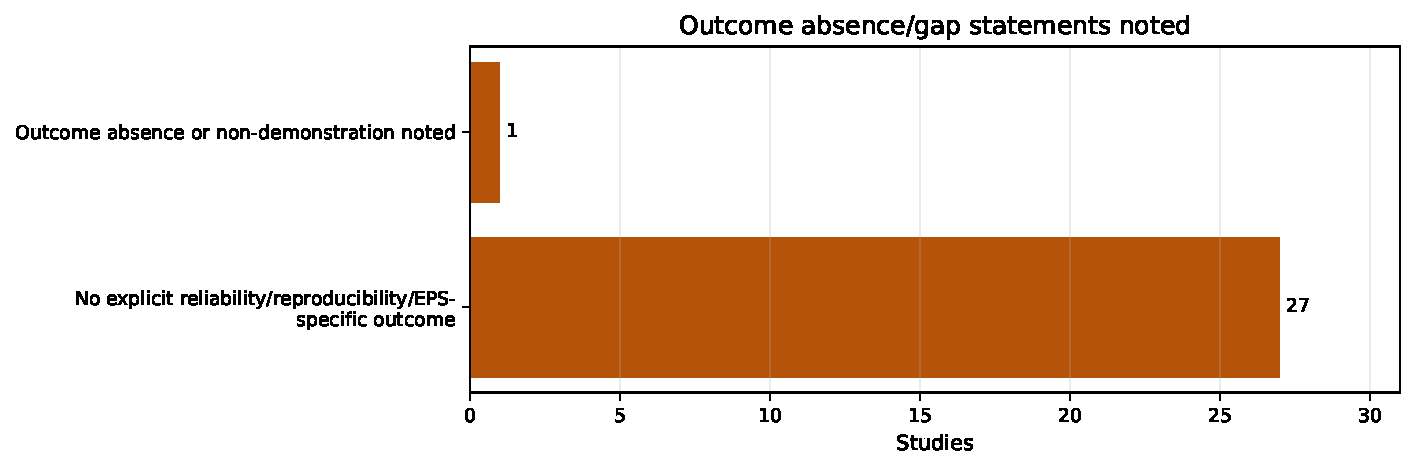
\includegraphics[width=0.72\linewidth]{outcome_gap_categories.pdf}
\caption{Outcome absence/gap categories explicitly noted in extraction bullets.}
\end{figure}

\begin{longtable}{p{0.48\linewidth}r p{0.34\linewidth}}
\toprule
Category & n & Study IDs \\
\midrule
\endfirsthead
\toprule Category & n & Study IDs \\ \midrule \endhead
Efficiency, automation, or reduced time/cost/effort & 32 & paper-0002, paper-0003, paper-0005, paper-0007, paper-0008, paper-0010, paper-0011, paper-0012, paper-0015, paper-0016, paper-0022, paper-0023, paper-0026, paper-0027, paper-0029, paper-0031, paper-0033, paper-0034, paper-0037, paper-0039, paper-0041, paper-0043, paper-0053, paper-0054, paper-0059, paper-0061, paper-0063, paper-0068, paper-0078, paper-0079, paper-0080, paper-0081 \\
Integration, interoperability, or data exchange & 32 & paper-0001, paper-0003, paper-0004, paper-0005, paper-0008, paper-0010, paper-0012, paper-0013, paper-0016, paper-0022, paper-0023, paper-0024, paper-0026, paper-0027, paper-0029, paper-0031, paper-0033, paper-0037, paper-0043, paper-0046, paper-0053, paper-0054, paper-0059, paper-0061, paper-0063, paper-0068, paper-0071, paper-0077, paper-0078, paper-0079, paper-0080, paper-0081 \\
Communication, collaboration, or stakeholder alignment & 30 & paper-0001, paper-0002, paper-0003, paper-0004, paper-0005, paper-0007, paper-0008, paper-0010, paper-0011, paper-0013, paper-0014, paper-0015, paper-0016, paper-0022, paper-0023, paper-0027, paper-0031, paper-0037, paper-0039, paper-0043, paper-0046, paper-0053, paper-0054, paper-0059, paper-0061, paper-0068, paper-0071, paper-0077, paper-0078, paper-0079 \\
Reuse, templates, standardization, or replicability & 27 & paper-0001, paper-0003, paper-0004, paper-0005, paper-0008, paper-0011, paper-0013, paper-0014, paper-0015, paper-0016, paper-0022, paper-0023, paper-0026, paper-0027, paper-0029, paper-0031, paper-0039, paper-0041, paper-0043, paper-0053, paper-0054, paper-0063, paper-0071, paper-0077, paper-0079, paper-0080, paper-0081 \\
Traceability, consistency, or single source of truth & 27 & paper-0001, paper-0002, paper-0004, paper-0005, paper-0007, paper-0013, paper-0016, paper-0022, paper-0023, paper-0026, paper-0027, paper-0029, paper-0031, paper-0034, paper-0037, paper-0041, paper-0043, paper-0046, paper-0054, paper-0059, paper-0063, paper-0071, paper-0077, paper-0078, paper-0079, paper-0080, paper-0081 \\
Simulation, trade-space, budget, or early analysis support & 25 & paper-0001, paper-0003, paper-0004, paper-0005, paper-0007, paper-0008, paper-0012, paper-0013, paper-0016, paper-0022, paper-0026, paper-0029, paper-0031, paper-0033, paper-0039, paper-0041, paper-0043, paper-0046, paper-0053, paper-0054, paper-0059, paper-0061, paper-0063, paper-0079, paper-0080 \\
Reliability, mission success, quality, risk, or robustness & 22 & paper-0002, paper-0003, paper-0007, paper-0008, paper-0010, paper-0011, paper-0012, paper-0013, paper-0014, paper-0023, paper-0034, paper-0039, paper-0041, paper-0043, paper-0053, paper-0054, paper-0061, paper-0063, paper-0071, paper-0078, paper-0079, paper-0080 \\
Verification, validation, test, or compliance support & 20 & paper-0001, paper-0003, paper-0004, paper-0008, paper-0010, paper-0013, paper-0015, paper-0023, paper-0033, paper-0034, paper-0039, paper-0043, paper-0053, paper-0059, paper-0061, paper-0063, paper-0071, paper-0077, paper-0079, paper-0080 \\
Documentation, configuration, or change management & 15 & paper-0002, paper-0003, paper-0008, paper-0016, paper-0023, paper-0031, paper-0033, paper-0037, paper-0041, paper-0046, paper-0053, paper-0059, paper-0063, paper-0078, paper-0080 \\
Openness, accessibility, or reproducibility & 11 & paper-0001, paper-0014, paper-0016, paper-0026, paper-0027, paper-0029, paper-0031, paper-0043, paper-0053, paper-0061, paper-0081 \\
\bottomrule
\end{longtable}

\subsection{How verification/validation was linked to models}
The most common verification-linkage categories are: V\&V packages, reviews, plans, or procedures (28), Parametric, constraint, budget, or resource checks (20), Executable simulation linked to the model (16), Requirements linked through satisfy/verify/trace relations (13), General MBSE V\&V statement only (8).  These are multi-label categories; for example, a study can have requirements traceability, parametric checks, and external tool coupling at the same time.

\begin{figure}[htbp]
\centering
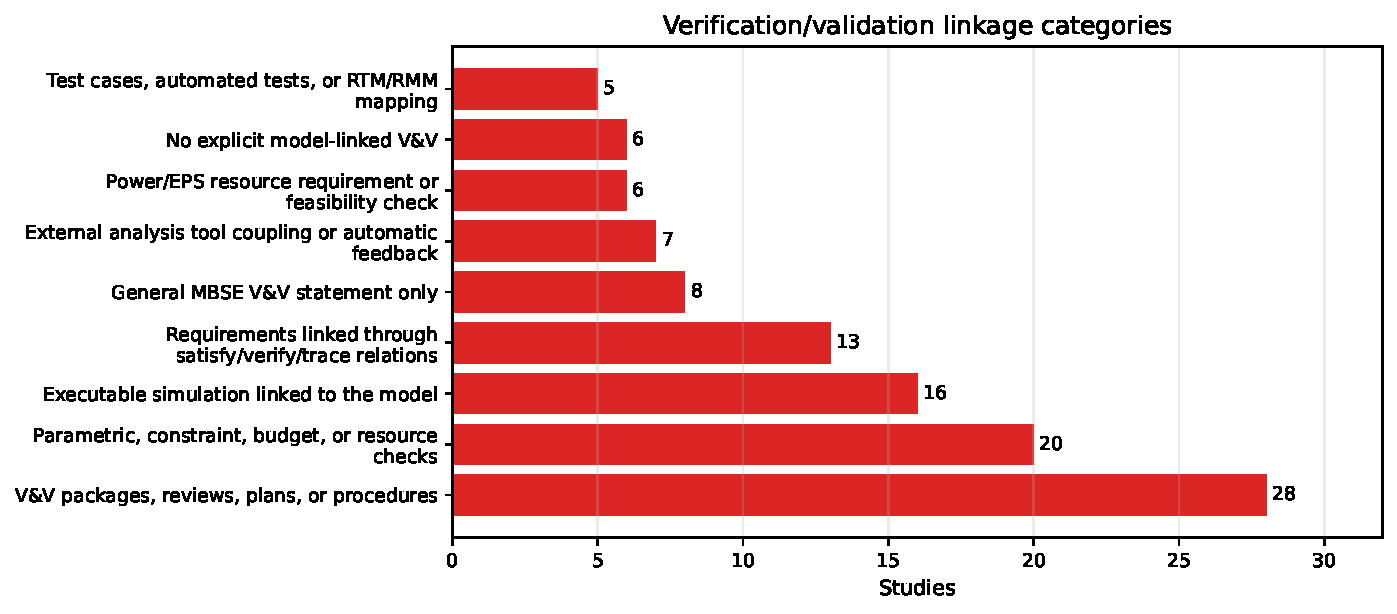
\includegraphics[width=0.92\linewidth]{vv_linkage_categories.pdf}
\caption{How verification/validation was linked to the model in the extractions.}
\end{figure}

\begin{longtable}{p{0.48\linewidth}r p{0.34\linewidth}}
\toprule
Category & n & Study IDs \\
\midrule
\endfirsthead
\toprule Category & n & Study IDs \\ \midrule \endhead
V\&V packages, reviews, plans, or procedures & 28 & paper-0003, paper-0004, paper-0005, paper-0007, paper-0008, paper-0010, paper-0011, paper-0013, paper-0014, paper-0015, paper-0016, paper-0023, paper-0024, paper-0031, paper-0033, paper-0034, paper-0037, paper-0039, paper-0041, paper-0043, paper-0053, paper-0059, paper-0061, paper-0071, paper-0077, paper-0078, paper-0080, paper-0081 \\
Parametric, constraint, budget, or resource checks & 20 & paper-0001, paper-0003, paper-0008, paper-0023, paper-0026, paper-0027, paper-0029, paper-0033, paper-0039, paper-0041, paper-0043, paper-0053, paper-0059, paper-0061, paper-0063, paper-0068, paper-0077, paper-0078, paper-0079, paper-0080 \\
Executable simulation linked to the model & 16 & paper-0001, paper-0003, paper-0005, paper-0010, paper-0011, paper-0027, paper-0029, paper-0033, paper-0041, paper-0043, paper-0053, paper-0059, paper-0077, paper-0078, paper-0079, paper-0080 \\
Requirements linked through satisfy/verify/trace relations & 13 & paper-0001, paper-0003, paper-0010, paper-0011, paper-0013, paper-0014, paper-0023, paper-0037, paper-0063, paper-0071, paper-0077, paper-0079, paper-0080 \\
General MBSE V\&V statement only & 8 & paper-0002, paper-0007, paper-0012, paper-0022, paper-0039, paper-0041, paper-0054, paper-0061 \\
External analysis tool coupling or automatic feedback & 7 & paper-0001, paper-0003, paper-0059, paper-0063, paper-0078, paper-0079, paper-0080 \\
Power/EPS resource requirement or feasibility check & 6 & paper-0001, paper-0008, paper-0043, paper-0053, paper-0059, paper-0077 \\
No explicit model-linked V\&V & 6 & paper-0002, paper-0012, paper-0024, paper-0029, paper-0046, paper-0068 \\
Test cases, automated tests, or RTM/RMM mapping & 5 & paper-0008, paper-0023, paper-0034, paper-0078, paper-0080 \\
\bottomrule
\end{longtable}

\subsection{Kinds of verification performed or proposed}
\begin{figure}[htbp]
\centering
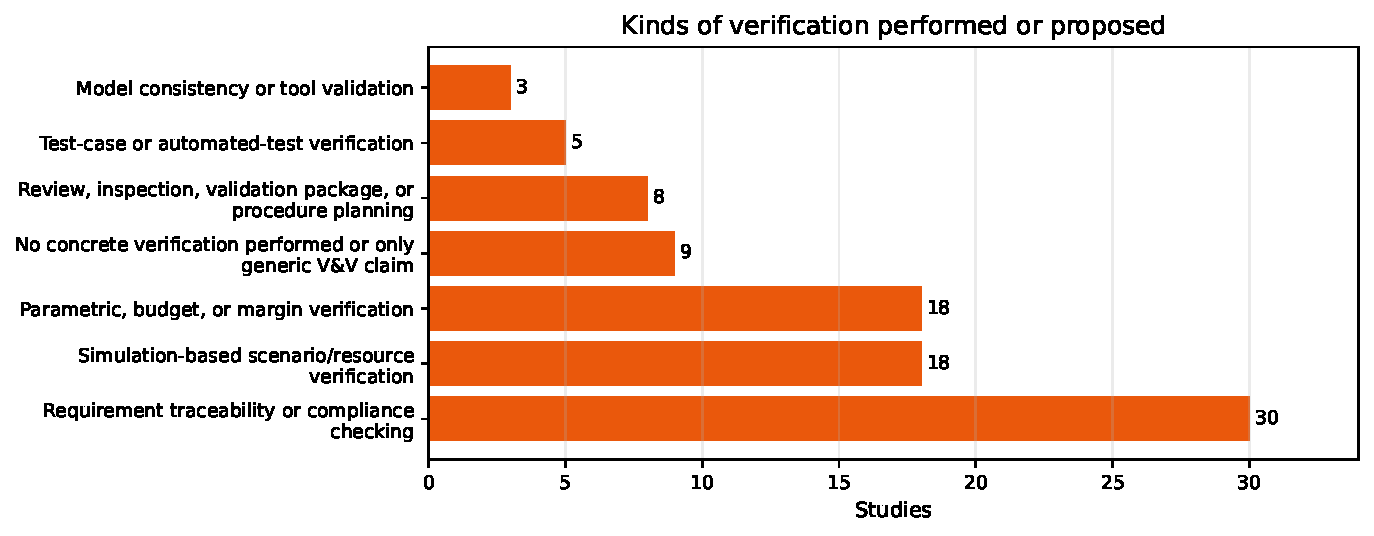
\includegraphics[width=0.92\linewidth]{verification_kind_categories.pdf}
\caption{Kinds of verification performed or proposed, derived from V\&V linkage and key-finding fields.}
\end{figure}

\begin{longtable}{p{0.48\linewidth}r p{0.34\linewidth}}
\toprule
Category & n & Study IDs \\
\midrule
\endfirsthead
\toprule Category & n & Study IDs \\ \midrule \endhead
Requirement traceability or compliance checking & 30 & paper-0001, paper-0002, paper-0003, paper-0004, paper-0007, paper-0008, paper-0011, paper-0013, paper-0014, paper-0016, paper-0022, paper-0023, paper-0026, paper-0027, paper-0029, paper-0031, paper-0033, paper-0034, paper-0037, paper-0039, paper-0043, paper-0046, paper-0053, paper-0054, paper-0059, paper-0063, paper-0077, paper-0078, paper-0079, paper-0080 \\
Simulation-based scenario/resource verification & 18 & paper-0001, paper-0003, paper-0005, paper-0008, paper-0010, paper-0015, paper-0023, paper-0027, paper-0029, paper-0033, paper-0034, paper-0041, paper-0043, paper-0053, paper-0054, paper-0059, paper-0078, paper-0079 \\
Parametric, budget, or margin verification & 18 & paper-0001, paper-0003, paper-0008, paper-0023, paper-0026, paper-0027, paper-0029, paper-0033, paper-0039, paper-0041, paper-0043, paper-0053, paper-0059, paper-0063, paper-0077, paper-0078, paper-0079, paper-0080 \\
No concrete verification performed or only generic V\&V claim & 9 & paper-0002, paper-0012, paper-0022, paper-0024, paper-0029, paper-0039, paper-0046, paper-0061, paper-0068 \\
Review, inspection, validation package, or procedure planning & 8 & paper-0005, paper-0011, paper-0013, paper-0014, paper-0015, paper-0023, paper-0077, paper-0081 \\
Test-case or automated-test verification & 5 & paper-0008, paper-0023, paper-0034, paper-0078, paper-0080 \\
Model consistency or tool validation & 3 & paper-0010, paper-0043, paper-0081 \\
\bottomrule
\end{longtable}

\section{Contributions and limitations}
The contribution taxonomy shows what each paper primarily added to the corpus.  The most frequent contribution categories are: Toolchain, data integration, or interoperability (40), Method, framework, process, or workflow (40), System-/mission-level nanosatellite model (39), Mission or case-study application (39), Simulation, trade study, executable analysis, or sizing (38).

\begin{figure}[htbp]
\centering
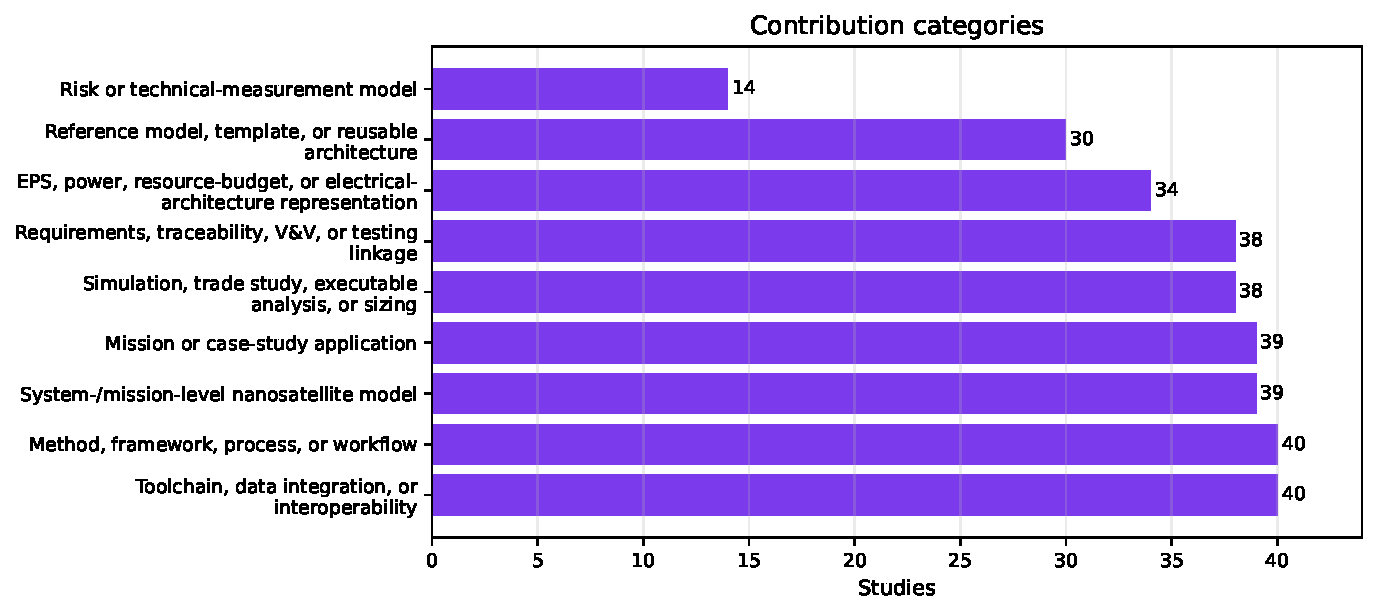
\includegraphics[width=0.92\linewidth]{contribution_categories.pdf}
\caption{Contribution categories derived from key findings, modeling scope, and tool/method fields.}
\end{figure}

\begin{longtable}{p{0.48\linewidth}r p{0.34\linewidth}}
\toprule
Category & n & Study IDs \\
\midrule
\endfirsthead
\toprule Category & n & Study IDs \\ \midrule \endhead
Toolchain, data integration, or interoperability & 40 & paper-0001, paper-0002, paper-0003, paper-0004, paper-0005, paper-0007, paper-0008, paper-0010, paper-0011, paper-0012, paper-0013, paper-0014, paper-0015, paper-0016, paper-0022, paper-0023, paper-0024, paper-0026, paper-0027, paper-0029, paper-0031, paper-0033, paper-0034, paper-0037, paper-0039, paper-0041, paper-0043, paper-0046, paper-0053, paper-0054, paper-0059, paper-0061, paper-0063, paper-0068, paper-0071, paper-0077, paper-0078, paper-0079, paper-0080, paper-0081 \\
Method, framework, process, or workflow & 40 & paper-0001, paper-0002, paper-0003, paper-0004, paper-0005, paper-0007, paper-0008, paper-0010, paper-0011, paper-0012, paper-0013, paper-0014, paper-0015, paper-0016, paper-0022, paper-0023, paper-0024, paper-0026, paper-0027, paper-0029, paper-0031, paper-0033, paper-0034, paper-0037, paper-0039, paper-0041, paper-0043, paper-0046, paper-0053, paper-0054, paper-0059, paper-0061, paper-0063, paper-0068, paper-0071, paper-0077, paper-0078, paper-0079, paper-0080, paper-0081 \\
System-/mission-level nanosatellite model & 39 & paper-0001, paper-0002, paper-0003, paper-0004, paper-0005, paper-0007, paper-0008, paper-0010, paper-0011, paper-0012, paper-0013, paper-0014, paper-0015, paper-0016, paper-0022, paper-0023, paper-0024, paper-0027, paper-0029, paper-0031, paper-0033, paper-0034, paper-0037, paper-0039, paper-0041, paper-0043, paper-0046, paper-0053, paper-0054, paper-0059, paper-0061, paper-0063, paper-0068, paper-0071, paper-0077, paper-0078, paper-0079, paper-0080, paper-0081 \\
Mission or case-study application & 39 & paper-0001, paper-0002, paper-0003, paper-0004, paper-0005, paper-0007, paper-0008, paper-0010, paper-0011, paper-0012, paper-0013, paper-0014, paper-0015, paper-0016, paper-0022, paper-0023, paper-0024, paper-0026, paper-0027, paper-0029, paper-0031, paper-0033, paper-0034, paper-0037, paper-0039, paper-0041, paper-0043, paper-0053, paper-0054, paper-0059, paper-0061, paper-0063, paper-0068, paper-0071, paper-0077, paper-0078, paper-0079, paper-0080, paper-0081 \\
Simulation, trade study, executable analysis, or sizing & 38 & paper-0001, paper-0002, paper-0003, paper-0004, paper-0005, paper-0007, paper-0008, paper-0010, paper-0011, paper-0012, paper-0013, paper-0014, paper-0015, paper-0016, paper-0022, paper-0023, paper-0024, paper-0026, paper-0027, paper-0029, paper-0031, paper-0033, paper-0034, paper-0037, paper-0039, paper-0041, paper-0043, paper-0046, paper-0053, paper-0054, paper-0059, paper-0061, paper-0063, paper-0077, paper-0078, paper-0079, paper-0080, paper-0081 \\
Requirements, traceability, V\&V, or testing linkage & 38 & paper-0001, paper-0002, paper-0003, paper-0004, paper-0005, paper-0007, paper-0008, paper-0010, paper-0011, paper-0012, paper-0013, paper-0014, paper-0015, paper-0016, paper-0022, paper-0023, paper-0026, paper-0027, paper-0029, paper-0031, paper-0033, paper-0034, paper-0037, paper-0039, paper-0041, paper-0043, paper-0046, paper-0053, paper-0054, paper-0059, paper-0061, paper-0063, paper-0071, paper-0077, paper-0078, paper-0079, paper-0080, paper-0081 \\
EPS, power, resource-budget, or electrical-architecture representation & 34 & paper-0001, paper-0003, paper-0004, paper-0005, paper-0007, paper-0008, paper-0011, paper-0012, paper-0013, paper-0014, paper-0015, paper-0016, paper-0022, paper-0023, paper-0026, paper-0027, paper-0029, paper-0031, paper-0033, paper-0037, paper-0039, paper-0041, paper-0043, paper-0046, paper-0053, paper-0054, paper-0059, paper-0061, paper-0071, paper-0077, paper-0078, paper-0079, paper-0080, paper-0081 \\
Reference model, template, or reusable architecture & 30 & paper-0001, paper-0002, paper-0003, paper-0004, paper-0005, paper-0007, paper-0008, paper-0011, paper-0012, paper-0013, paper-0014, paper-0015, paper-0016, paper-0022, paper-0023, paper-0026, paper-0029, paper-0031, paper-0033, paper-0037, paper-0039, paper-0053, paper-0054, paper-0061, paper-0068, paper-0071, paper-0077, paper-0079, paper-0080, paper-0081 \\
Risk or technical-measurement model & 14 & paper-0002, paper-0007, paper-0008, paper-0010, paper-0011, paper-0013, paper-0014, paper-0022, paper-0054, paper-0061, paper-0071, paper-0077, paper-0078, paper-0080 \\
\bottomrule
\end{longtable}

Limitations are also multi-label.  The most frequent limitation categories are: Prototype, incomplete maturity, or future work (31), Limited scope, single case, or partial subsystem/mode coverage (24), No quantitative evaluation, weak validation, or no threats discussion (24), Data, model-quality, source, or assumption limitation (18), Tool dependency, interoperability, licensing, or learning curve (16).  Several studies do not provide formal limitations/threats-to-validity discussions; those are explicitly separated rather than silently ignored.

\begin{figure}[htbp]
\centering
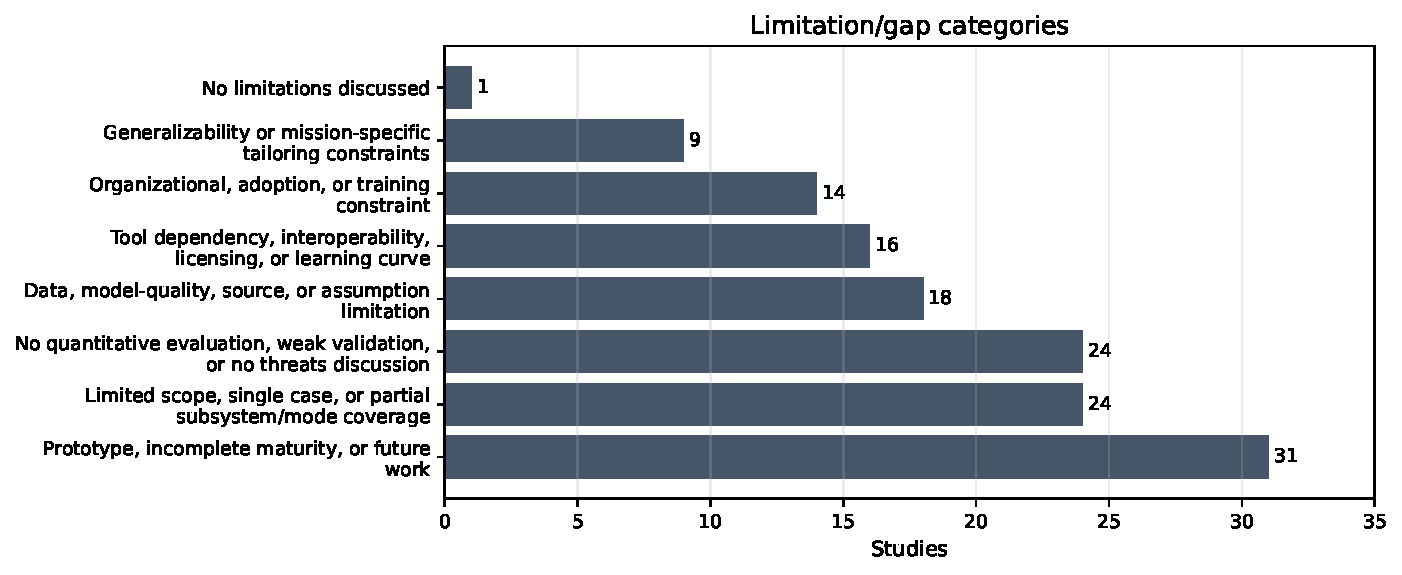
\includegraphics[width=0.92\linewidth]{limitation_categories.pdf}
\caption{Limitation/gap categories derived from the standardized limitation fields.}
\end{figure}

\begin{longtable}{p{0.48\linewidth}r p{0.34\linewidth}}
\toprule
Category & n & Study IDs \\
\midrule
\endfirsthead
\toprule Category & n & Study IDs \\ \midrule \endhead
Prototype, incomplete maturity, or future work & 31 & paper-0001, paper-0002, paper-0003, paper-0004, paper-0005, paper-0008, paper-0011, paper-0013, paper-0016, paper-0022, paper-0023, paper-0024, paper-0026, paper-0027, paper-0029, paper-0031, paper-0033, paper-0034, paper-0037, paper-0041, paper-0043, paper-0046, paper-0054, paper-0061, paper-0063, paper-0068, paper-0077, paper-0078, paper-0079, paper-0080, paper-0081 \\
Limited scope, single case, or partial subsystem/mode coverage & 24 & paper-0001, paper-0002, paper-0003, paper-0004, paper-0008, paper-0012, paper-0016, paper-0022, paper-0023, paper-0024, paper-0026, paper-0027, paper-0029, paper-0039, paper-0041, paper-0043, paper-0046, paper-0053, paper-0059, paper-0061, paper-0063, paper-0071, paper-0078, paper-0079 \\
No quantitative evaluation, weak validation, or no threats discussion & 24 & paper-0001, paper-0002, paper-0004, paper-0007, paper-0008, paper-0010, paper-0011, paper-0013, paper-0015, paper-0016, paper-0022, paper-0023, paper-0029, paper-0031, paper-0033, paper-0034, paper-0039, paper-0041, paper-0043, paper-0046, paper-0059, paper-0061, paper-0068, paper-0071 \\
Data, model-quality, source, or assumption limitation & 18 & paper-0001, paper-0002, paper-0003, paper-0004, paper-0005, paper-0008, paper-0010, paper-0012, paper-0024, paper-0026, paper-0027, paper-0029, paper-0033, paper-0037, paper-0039, paper-0043, paper-0046, paper-0061 \\
Tool dependency, interoperability, licensing, or learning curve & 16 & paper-0003, paper-0004, paper-0008, paper-0014, paper-0023, paper-0027, paper-0029, paper-0039, paper-0041, paper-0046, paper-0059, paper-0061, paper-0063, paper-0071, paper-0080, paper-0081 \\
Organizational, adoption, or training constraint & 14 & paper-0003, paper-0005, paper-0008, paper-0011, paper-0012, paper-0015, paper-0022, paper-0037, paper-0039, paper-0046, paper-0071, paper-0077, paper-0078, paper-0080 \\
Generalizability or mission-specific tailoring constraints & 9 & paper-0012, paper-0013, paper-0015, paper-0016, paper-0022, paper-0029, paper-0039, paper-0054, paper-0077 \\
No limitations discussed & 1 & paper-0053 \\
\bottomrule
\end{longtable}

\clearpage
\section{Study-level contribution and limitation map}
The following landscape table supports paper-by-paper inspection of what each extraction contributed and what limitations/gaps were recorded.

\begin{landscape}
\scriptsize
\begin{longtable}{p{0.08\linewidth}p{0.20\linewidth}p{0.31\linewidth}p{0.31\linewidth}}
\toprule Study & Short title & Contribution categories & Limitation categories \\
\midrule\endfirsthead
\toprule Study & Short title & Contribution categories & Limitation categories \\ \midrule\endhead
paper-0003 & Model Based Systems Engineering (MBSE) Applied to Radio... & EPS, power, resource-budget, or electrical-architecture representation; Method, framework, process, or workflow; Mission or case-study application; Reference model, template, or reusable architecture; Requirements, traceability, V\&V, or testing linkage; Simulation, trade study, executable analysis, or sizing; System-/mission-level nanosatellite model; Toolchain, data integration, or interoperability & Data, model-quality, source, or assumption limitation; Limited scope, single case, or partial subsystem/mode coverage; Organizational, adoption, or training constraint; Prototype, incomplete maturity, or future work; Tool dependency, interoperability, licensing, or learning curve \\
paper-0001 & Integrated Model-Based Systems Engineering (MBSE)... & EPS, power, resource-budget, or electrical-architecture representation; Method, framework, process, or workflow; Mission or case-study application; Reference model, template, or reusable architecture; Requirements, traceability, V\&V, or testing linkage; Simulation, trade study, executable analysis, or sizing; System-/mission-level nanosatellite model; Toolchain, data integration, or interoperability & Data, model-quality, source, or assumption limitation; Limited scope, single case, or partial subsystem/mode coverage; No quantitative evaluation, weak validation, or no threats discussion; Prototype, incomplete maturity, or future work \\
paper-0008 & Enterprise modeling for CubeSats & EPS, power, resource-budget, or electrical-architecture representation; Method, framework, process, or workflow; Mission or case-study application; Reference model, template, or reusable architecture; Requirements, traceability, V\&V, or testing linkage; Risk or technical-measurement model; Simulation, trade study, executable analysis, or sizing; System-/mission-level nanosatellite model; Toolchain, data integration, or interoperability & Data, model-quality, source, or assumption limitation; Limited scope, single case, or partial subsystem/mode coverage; No quantitative evaluation, weak validation, or no threats discussion; Organizational, adoption, or training constraint; Prototype, incomplete maturity, or future work; Tool dependency, interoperability, licensing, or learning curve \\
paper-0010 & Small Satellite Systems Design Methodology: A Formal... & Method, framework, process, or workflow; Mission or case-study application; Requirements, traceability, V\&V, or testing linkage; Risk or technical-measurement model; Simulation, trade study, executable analysis, or sizing; System-/mission-level nanosatellite model; Toolchain, data integration, or interoperability & Data, model-quality, source, or assumption limitation; No quantitative evaluation, weak validation, or no threats discussion \\
paper-0012 & Rapid model-based inter-disciplinary design of a... & EPS, power, resource-budget, or electrical-architecture representation; Method, framework, process, or workflow; Mission or case-study application; Reference model, template, or reusable architecture; Requirements, traceability, V\&V, or testing linkage; Simulation, trade study, executable analysis, or sizing; System-/mission-level nanosatellite model; Toolchain, data integration, or interoperability & Data, model-quality, source, or assumption limitation; Generalizability or mission-specific tailoring constraints; Limited scope, single case, or partial subsystem/mode coverage; Organizational, adoption, or training constraint \\
paper-0079 & Model-based systems engineering to support the... & EPS, power, resource-budget, or electrical-architecture representation; Method, framework, process, or workflow; Mission or case-study application; Reference model, template, or reusable architecture; Requirements, traceability, V\&V, or testing linkage; Simulation, trade study, executable analysis, or sizing; System-/mission-level nanosatellite model; Toolchain, data integration, or interoperability & Limited scope, single case, or partial subsystem/mode coverage; Prototype, incomplete maturity, or future work \\
paper-0004 & Developing a CubeSat Model-Based System Engineering... & EPS, power, resource-budget, or electrical-architecture representation; Method, framework, process, or workflow; Mission or case-study application; Reference model, template, or reusable architecture; Requirements, traceability, V\&V, or testing linkage; Simulation, trade study, executable analysis, or sizing; System-/mission-level nanosatellite model; Toolchain, data integration, or interoperability & Data, model-quality, source, or assumption limitation; Limited scope, single case, or partial subsystem/mode coverage; No quantitative evaluation, weak validation, or no threats discussion; Prototype, incomplete maturity, or future work; Tool dependency, interoperability, licensing, or learning curve \\
paper-0022 & CubeSat Model-Based System Engineering (MBSE) Reference... & EPS, power, resource-budget, or electrical-architecture representation; Method, framework, process, or workflow; Mission or case-study application; Reference model, template, or reusable architecture; Requirements, traceability, V\&V, or testing linkage; Risk or technical-measurement model; Simulation, trade study, executable analysis, or sizing; System-/mission-level nanosatellite model; Toolchain, data integration, or interoperability & Generalizability or mission-specific tailoring constraints; Limited scope, single case, or partial subsystem/mode coverage; No quantitative evaluation, weak validation, or no threats discussion; Organizational, adoption, or training constraint; Prototype, incomplete maturity, or future work \\
paper-0016 & Developing a CubeSat Model-Based System Engineering... & EPS, power, resource-budget, or electrical-architecture representation; Method, framework, process, or workflow; Mission or case-study application; Reference model, template, or reusable architecture; Requirements, traceability, V\&V, or testing linkage; Simulation, trade study, executable analysis, or sizing; System-/mission-level nanosatellite model; Toolchain, data integration, or interoperability & Generalizability or mission-specific tailoring constraints; Limited scope, single case, or partial subsystem/mode coverage; No quantitative evaluation, weak validation, or no threats discussion; Prototype, incomplete maturity, or future work \\
paper-0031 & CubeSat Model-Based System Engineering (MBSE) reference... & EPS, power, resource-budget, or electrical-architecture representation; Method, framework, process, or workflow; Mission or case-study application; Reference model, template, or reusable architecture; Requirements, traceability, V\&V, or testing linkage; Simulation, trade study, executable analysis, or sizing; System-/mission-level nanosatellite model; Toolchain, data integration, or interoperability & No quantitative evaluation, weak validation, or no threats discussion; Prototype, incomplete maturity, or future work \\
paper-0002 & A Model-Based Systems Engineering (MBSE) Approach for... & Method, framework, process, or workflow; Mission or case-study application; Reference model, template, or reusable architecture; Requirements, traceability, V\&V, or testing linkage; Risk or technical-measurement model; Simulation, trade study, executable analysis, or sizing; System-/mission-level nanosatellite model; Toolchain, data integration, or interoperability & Data, model-quality, source, or assumption limitation; Limited scope, single case, or partial subsystem/mode coverage; No quantitative evaluation, weak validation, or no threats discussion; Prototype, incomplete maturity, or future work \\
paper-0005 & Developing a CubeSat Model-Based System Engineering... & EPS, power, resource-budget, or electrical-architecture representation; Method, framework, process, or workflow; Mission or case-study application; Reference model, template, or reusable architecture; Requirements, traceability, V\&V, or testing linkage; Simulation, trade study, executable analysis, or sizing; System-/mission-level nanosatellite model; Toolchain, data integration, or interoperability & Data, model-quality, source, or assumption limitation; Organizational, adoption, or training constraint; Prototype, incomplete maturity, or future work \\
paper-0015 & Validation and Verification of MBSE-compliant CubeSat... & EPS, power, resource-budget, or electrical-architecture representation; Method, framework, process, or workflow; Mission or case-study application; Reference model, template, or reusable architecture; Requirements, traceability, V\&V, or testing linkage; Simulation, trade study, executable analysis, or sizing; System-/mission-level nanosatellite model; Toolchain, data integration, or interoperability & Generalizability or mission-specific tailoring constraints; No quantitative evaluation, weak validation, or no threats discussion; Organizational, adoption, or training constraint \\
paper-0007 & A model-based systems engineering approach for... & EPS, power, resource-budget, or electrical-architecture representation; Method, framework, process, or workflow; Mission or case-study application; Reference model, template, or reusable architecture; Requirements, traceability, V\&V, or testing linkage; Risk or technical-measurement model; Simulation, trade study, executable analysis, or sizing; System-/mission-level nanosatellite model; Toolchain, data integration, or interoperability & No quantitative evaluation, weak validation, or no threats discussion \\
paper-0013 & Developing a CubeSat Model-Based System Engineering... & EPS, power, resource-budget, or electrical-architecture representation; Method, framework, process, or workflow; Mission or case-study application; Reference model, template, or reusable architecture; Requirements, traceability, V\&V, or testing linkage; Risk or technical-measurement model; Simulation, trade study, executable analysis, or sizing; System-/mission-level nanosatellite model; Toolchain, data integration, or interoperability & Generalizability or mission-specific tailoring constraints; No quantitative evaluation, weak validation, or no threats discussion; Prototype, incomplete maturity, or future work \\
paper-0080 & Application of Model-Based Systems Engineering in Small... & EPS, power, resource-budget, or electrical-architecture representation; Method, framework, process, or workflow; Mission or case-study application; Reference model, template, or reusable architecture; Requirements, traceability, V\&V, or testing linkage; Risk or technical-measurement model; Simulation, trade study, executable analysis, or sizing; System-/mission-level nanosatellite model; Toolchain, data integration, or interoperability & Organizational, adoption, or training constraint; Prototype, incomplete maturity, or future work; Tool dependency, interoperability, licensing, or learning curve \\
paper-0034 & Requirements Modeling Language and Automated Testing... & Method, framework, process, or workflow; Mission or case-study application; Requirements, traceability, V\&V, or testing linkage; Simulation, trade study, executable analysis, or sizing; System-/mission-level nanosatellite model; Toolchain, data integration, or interoperability & No quantitative evaluation, weak validation, or no threats discussion; Prototype, incomplete maturity, or future work \\
paper-0077 & Developing a CubeSat System MBSE Reference Model –... & EPS, power, resource-budget, or electrical-architecture representation; Method, framework, process, or workflow; Mission or case-study application; Reference model, template, or reusable architecture; Requirements, traceability, V\&V, or testing linkage; Risk or technical-measurement model; Simulation, trade study, executable analysis, or sizing; System-/mission-level nanosatellite model; Toolchain, data integration, or interoperability & Generalizability or mission-specific tailoring constraints; Organizational, adoption, or training constraint; Prototype, incomplete maturity, or future work \\
paper-0011 & Development and Application of the CubeSat System... & EPS, power, resource-budget, or electrical-architecture representation; Method, framework, process, or workflow; Mission or case-study application; Reference model, template, or reusable architecture; Requirements, traceability, V\&V, or testing linkage; Risk or technical-measurement model; Simulation, trade study, executable analysis, or sizing; System-/mission-level nanosatellite model; Toolchain, data integration, or interoperability & No quantitative evaluation, weak validation, or no threats discussion; Organizational, adoption, or training constraint; Prototype, incomplete maturity, or future work \\
paper-0024 & Analysis of MBSE/PLM Integration: From Conceptual... & Method, framework, process, or workflow; Mission or case-study application; Simulation, trade study, executable analysis, or sizing; System-/mission-level nanosatellite model; Toolchain, data integration, or interoperability & Data, model-quality, source, or assumption limitation; Limited scope, single case, or partial subsystem/mode coverage; Prototype, incomplete maturity, or future work \\
paper-0039 & Applying a Model-Based Approach to Develop a... & EPS, power, resource-budget, or electrical-architecture representation; Method, framework, process, or workflow; Mission or case-study application; Reference model, template, or reusable architecture; Requirements, traceability, V\&V, or testing linkage; Simulation, trade study, executable analysis, or sizing; System-/mission-level nanosatellite model; Toolchain, data integration, or interoperability & Data, model-quality, source, or assumption limitation; Generalizability or mission-specific tailoring constraints; Limited scope, single case, or partial subsystem/mode coverage; No quantitative evaluation, weak validation, or no threats discussion; Organizational, adoption, or training constraint; Tool dependency, interoperability, licensing, or learning curve \\
paper-0068 & Digital Engineering Information Exchange Model for... & Method, framework, process, or workflow; Mission or case-study application; Reference model, template, or reusable architecture; System-/mission-level nanosatellite model; Toolchain, data integration, or interoperability & No quantitative evaluation, weak validation, or no threats discussion; Prototype, incomplete maturity, or future work \\
paper-0014 & Mission Engineering and the CubeSat System Reference Model & EPS, power, resource-budget, or electrical-architecture representation; Method, framework, process, or workflow; Mission or case-study application; Reference model, template, or reusable architecture; Requirements, traceability, V\&V, or testing linkage; Risk or technical-measurement model; Simulation, trade study, executable analysis, or sizing; System-/mission-level nanosatellite model; Toolchain, data integration, or interoperability & Tool dependency, interoperability, licensing, or learning curve \\
paper-0033 & Towards Simulation of CubeSat Operational Scenarios... & EPS, power, resource-budget, or electrical-architecture representation; Method, framework, process, or workflow; Mission or case-study application; Reference model, template, or reusable architecture; Requirements, traceability, V\&V, or testing linkage; Simulation, trade study, executable analysis, or sizing; System-/mission-level nanosatellite model; Toolchain, data integration, or interoperability & Data, model-quality, source, or assumption limitation; No quantitative evaluation, weak validation, or no threats discussion; Prototype, incomplete maturity, or future work \\
paper-0027 & MBSE Challenges in the Concurrent Preliminary Design of... & EPS, power, resource-budget, or electrical-architecture representation; Method, framework, process, or workflow; Mission or case-study application; Requirements, traceability, V\&V, or testing linkage; Simulation, trade study, executable analysis, or sizing; System-/mission-level nanosatellite model; Toolchain, data integration, or interoperability & Data, model-quality, source, or assumption limitation; Limited scope, single case, or partial subsystem/mode coverage; Prototype, incomplete maturity, or future work; Tool dependency, interoperability, licensing, or learning curve \\
paper-0046 & Investigating the Effectiveness of a Causal MBSE... & EPS, power, resource-budget, or electrical-architecture representation; Method, framework, process, or workflow; Requirements, traceability, V\&V, or testing linkage; Simulation, trade study, executable analysis, or sizing; System-/mission-level nanosatellite model; Toolchain, data integration, or interoperability & Data, model-quality, source, or assumption limitation; Limited scope, single case, or partial subsystem/mode coverage; No quantitative evaluation, weak validation, or no threats discussion; Organizational, adoption, or training constraint; Prototype, incomplete maturity, or future work; Tool dependency, interoperability, licensing, or learning curve \\
paper-0071 & A Model-Based Approach to Risk Management for RVSAT-1:... & EPS, power, resource-budget, or electrical-architecture representation; Method, framework, process, or workflow; Mission or case-study application; Reference model, template, or reusable architecture; Requirements, traceability, V\&V, or testing linkage; Risk or technical-measurement model; System-/mission-level nanosatellite model; Toolchain, data integration, or interoperability & Limited scope, single case, or partial subsystem/mode coverage; No quantitative evaluation, weak validation, or no threats discussion; Organizational, adoption, or training constraint; Tool dependency, interoperability, licensing, or learning curve \\
paper-0026 & Open-source CubeSat MBSE Approach to Address... & EPS, power, resource-budget, or electrical-architecture representation; Method, framework, process, or workflow; Mission or case-study application; Reference model, template, or reusable architecture; Requirements, traceability, V\&V, or testing linkage; Simulation, trade study, executable analysis, or sizing; Toolchain, data integration, or interoperability & Data, model-quality, source, or assumption limitation; Limited scope, single case, or partial subsystem/mode coverage; Prototype, incomplete maturity, or future work \\
paper-0037 & Model Based Systems Engineering with a Docs-as-Code... & EPS, power, resource-budget, or electrical-architecture representation; Method, framework, process, or workflow; Mission or case-study application; Reference model, template, or reusable architecture; Requirements, traceability, V\&V, or testing linkage; Simulation, trade study, executable analysis, or sizing; System-/mission-level nanosatellite model; Toolchain, data integration, or interoperability & Data, model-quality, source, or assumption limitation; Organizational, adoption, or training constraint; Prototype, incomplete maturity, or future work \\
paper-0063 & Development of a Nanosatellite System Modeling... & Method, framework, process, or workflow; Mission or case-study application; Requirements, traceability, V\&V, or testing linkage; Simulation, trade study, executable analysis, or sizing; System-/mission-level nanosatellite model; Toolchain, data integration, or interoperability & Limited scope, single case, or partial subsystem/mode coverage; Prototype, incomplete maturity, or future work; Tool dependency, interoperability, licensing, or learning curve \\
paper-0023 & Effective Model-Based Systems Engineering framework for... & EPS, power, resource-budget, or electrical-architecture representation; Method, framework, process, or workflow; Mission or case-study application; Reference model, template, or reusable architecture; Requirements, traceability, V\&V, or testing linkage; Simulation, trade study, executable analysis, or sizing; System-/mission-level nanosatellite model; Toolchain, data integration, or interoperability & Limited scope, single case, or partial subsystem/mode coverage; No quantitative evaluation, weak validation, or no threats discussion; Prototype, incomplete maturity, or future work; Tool dependency, interoperability, licensing, or learning curve \\
paper-0029 & Open-Source Data Formalization through Model-Based... & EPS, power, resource-budget, or electrical-architecture representation; Method, framework, process, or workflow; Mission or case-study application; Reference model, template, or reusable architecture; Requirements, traceability, V\&V, or testing linkage; Simulation, trade study, executable analysis, or sizing; System-/mission-level nanosatellite model; Toolchain, data integration, or interoperability & Data, model-quality, source, or assumption limitation; Generalizability or mission-specific tailoring constraints; Limited scope, single case, or partial subsystem/mode coverage; No quantitative evaluation, weak validation, or no threats discussion; Prototype, incomplete maturity, or future work; Tool dependency, interoperability, licensing, or learning curve \\
paper-0059 & An Implementation of Integrated Approach in Product... & EPS, power, resource-budget, or electrical-architecture representation; Method, framework, process, or workflow; Mission or case-study application; Requirements, traceability, V\&V, or testing linkage; Simulation, trade study, executable analysis, or sizing; System-/mission-level nanosatellite model; Toolchain, data integration, or interoperability & Limited scope, single case, or partial subsystem/mode coverage; No quantitative evaluation, weak validation, or no threats discussion; Tool dependency, interoperability, licensing, or learning curve \\
paper-0061 & Concurrent Model-Based Approach for CubeSat Mission Design & EPS, power, resource-budget, or electrical-architecture representation; Method, framework, process, or workflow; Mission or case-study application; Reference model, template, or reusable architecture; Requirements, traceability, V\&V, or testing linkage; Risk or technical-measurement model; Simulation, trade study, executable analysis, or sizing; System-/mission-level nanosatellite model; Toolchain, data integration, or interoperability & Data, model-quality, source, or assumption limitation; Limited scope, single case, or partial subsystem/mode coverage; No quantitative evaluation, weak validation, or no threats discussion; Prototype, incomplete maturity, or future work; Tool dependency, interoperability, licensing, or learning curve \\
paper-0078 & Preliminary Design of Satellite Systems through the... & EPS, power, resource-budget, or electrical-architecture representation; Method, framework, process, or workflow; Mission or case-study application; Requirements, traceability, V\&V, or testing linkage; Risk or technical-measurement model; Simulation, trade study, executable analysis, or sizing; System-/mission-level nanosatellite model; Toolchain, data integration, or interoperability & Limited scope, single case, or partial subsystem/mode coverage; Organizational, adoption, or training constraint; Prototype, incomplete maturity, or future work \\
paper-0041 & Applying Model-Based Systems Engineering on CubeSat... & EPS, power, resource-budget, or electrical-architecture representation; Method, framework, process, or workflow; Mission or case-study application; Requirements, traceability, V\&V, or testing linkage; Simulation, trade study, executable analysis, or sizing; System-/mission-level nanosatellite model; Toolchain, data integration, or interoperability & Limited scope, single case, or partial subsystem/mode coverage; No quantitative evaluation, weak validation, or no threats discussion; Prototype, incomplete maturity, or future work; Tool dependency, interoperability, licensing, or learning curve \\
paper-0043 & Towards a Unified Modeling and Simulation Framework for... & EPS, power, resource-budget, or electrical-architecture representation; Method, framework, process, or workflow; Mission or case-study application; Requirements, traceability, V\&V, or testing linkage; Simulation, trade study, executable analysis, or sizing; System-/mission-level nanosatellite model; Toolchain, data integration, or interoperability & Data, model-quality, source, or assumption limitation; Limited scope, single case, or partial subsystem/mode coverage; No quantitative evaluation, weak validation, or no threats discussion; Prototype, incomplete maturity, or future work \\
paper-0053 & CONCURRENT ENGINEERING PROCESS FOR ELECTRICAL... & EPS, power, resource-budget, or electrical-architecture representation; Method, framework, process, or workflow; Mission or case-study application; Reference model, template, or reusable architecture; Requirements, traceability, V\&V, or testing linkage; Simulation, trade study, executable analysis, or sizing; System-/mission-level nanosatellite model; Toolchain, data integration, or interoperability & Limited scope, single case, or partial subsystem/mode coverage; No limitations discussed \\
paper-0054 & Integrating Model-Based Systems Engineering into... & EPS, power, resource-budget, or electrical-architecture representation; Method, framework, process, or workflow; Mission or case-study application; Reference model, template, or reusable architecture; Requirements, traceability, V\&V, or testing linkage; Risk or technical-measurement model; Simulation, trade study, executable analysis, or sizing; System-/mission-level nanosatellite model; Toolchain, data integration, or interoperability & Generalizability or mission-specific tailoring constraints; Prototype, incomplete maturity, or future work \\
paper-0081 & Automating Object-Oriented Functional Modeling for... & EPS, power, resource-budget, or electrical-architecture representation; Method, framework, process, or workflow; Mission or case-study application; Reference model, template, or reusable architecture; Requirements, traceability, V\&V, or testing linkage; Simulation, trade study, executable analysis, or sizing; System-/mission-level nanosatellite model; Toolchain, data integration, or interoperability & Prototype, incomplete maturity, or future work; Tool dependency, interoperability, licensing, or learning curve \\
\bottomrule\end{longtable}
\end{landscape}

\section{Generated artifacts and reproducibility}
From the repository root, this report is regenerated by running:
\begin{verbatim}
python3 SLR/SLR1/scoping-review/scripts/generate_extraction_report.py
\end{verbatim}
The script writes the figures under \texttt{SLR/SLR1/scoping-review/figures/}, tabular derived data under \texttt{SLR/SLR1/scoping-review/data/}, and this LaTeX file at \texttt{SLR/SLR1/scoping-review/scoping-review.tex}.  The deterministic category rules are persisted in the script.

\end{document}
